\section{Results}
\label{sec:Results}

\fix{Nathan and Ron}

\subsection{Experimental Setup}

All experiments were performed on the Cielo supercomputer housed at Los Alamos
National Laboratory.  Cielo is an 1,840-node Cray XE6 resource for the Advanced
Simulation and Computing (ASC) program and is jointly managed by Sandia National 
Laboratories and Los Alamos National Laboratories under the New Mexico
Alliance for Computing at Extreme Scale (ACES) project.  Each node contains
two AMD Opteron 6100 (Magny-Cours) 8-way processor chips for a total of 16 cores
per node.  Each core has a peak computational speed of 2.6 GHz, leading to a total 
theoretical peak of 1.37 Petaflops for the machine. The compute nodes each
have 32 GB of memory.  The interconnect consists of a proprietary Cray Gemini
Network with a 3D Torus topology and has a peak throughput rate of 6 GB/s/link. 

The experiments in this report include strong scaling results for four different
CTH applications: an application that writes spyplot files, representing the traditional 
post-processing approach; an application that uses a Nessie servivce to provide \intransit
ParaView analysis; and two applications that perform ParaView \insitu analysis.  The first 
\insitu application, labeled \emph{\insitu (untuned)}, uses an algorithm that does not scale.
The second \insitu application, labeled \emph{\insitu (tuned)}, uses a more
scalable implementation of the same algorithm.  

%%%%%%%%%%%%%%%%%%%%%% -- table ---
\begin{table}

\caption{Scaling Overview}
\label{tab:ScalingOverview}

\centering{}%
\begin{tabular}{|c|c|c|}
\hline 
Data Set Size (blocks) & Client Ranks (16 cores/node) & Server Nodes (2, 4, and 8 cores/node)\tabularnewline
\hline 
\hline 
33k & 128, 256, 512, 1024 & 2\tabularnewline
\hline 
220k & 1024, 2048, 4096, 8192 & 16\tabularnewline
\hline 
1.5m & 4096, 8192, 16384, 32768 & 128\tabularnewline
\hline 
\end{tabular}
\end{table}

%%%%%%%%%%%%%%%%%%%%%% -- table ---

For each application, we run strong scaling experiments for three different datasets.  
Table~\ref{tab:ScalingOvewview} shows the range of core sizes used for the various
experiments.  The objective is run experiments with datasets representative of real
production runs.  The number of nodes/cores used is limited by amount of memory required
for a particular experiment.  


NEED MORE... WILL FINISH TOMORROW


\subsection{Total Runtime Measurements}


\subsection{Per Cycle Timings}





The following plots provide measured values of total runtime for each of the 

Total runtime is the ultimate measure of the performance when comparing 
approaches.  


\subsection{Memory}
The following memory plots were taken by examining free memory on the nodes
using /proc/meminfo.  Measuring free memory is conservative because it also
accounts for caches and buffers, so although you may run out of free memory in
a system, the execution will not immediately fail due to memory freed from
those other sources.  However, these are an indication of the worst case
possible.  On Cielo there are 16 cores per node and in each case the nodes were
 loaded with 16 MPI ranks executing the statically linked executable.  

In order to understand CTH memory usage results, it is important to note that
CTH preallocates memory based on a value for ``max number of blocks'' provided
through the input deck.  Because of this, CTH memory usage is highly impacted
by the user specification.  In this case we ran the results with what we
believe are reasonable values for ``max number of blocks'' given the size of the
problem.  Figure~\ref{fig:MaxBlocks} shows the corresponding max blocks for
each run.

\begin{figure}[htb]
  \centering
  \includegraphics[width=\linewidth]{figures/MaxNumberOfBlocks}
  \caption{A plot of the ``max number of blocks'' parameter supplied to CTH for each run.}
  \label{fig:MaxBlocks}
\end{figure}

Figure~\ref{fig:MemoryUsageAll} provides an overview of all memory
measurements taken for the system.  The memory taken by CTH is quite flat,
as expected, for each run.  However, even though the size of the mesh
changes throughout the simulation, the memory overhead for \insitu and
\intransit runs changes only moderately.  Thus, for the rest of the results
analysis, we summarize all measurements as simply the maximum value, which
is a reasonable representation of all values.

\begin{figure}[htb]
  \centering
  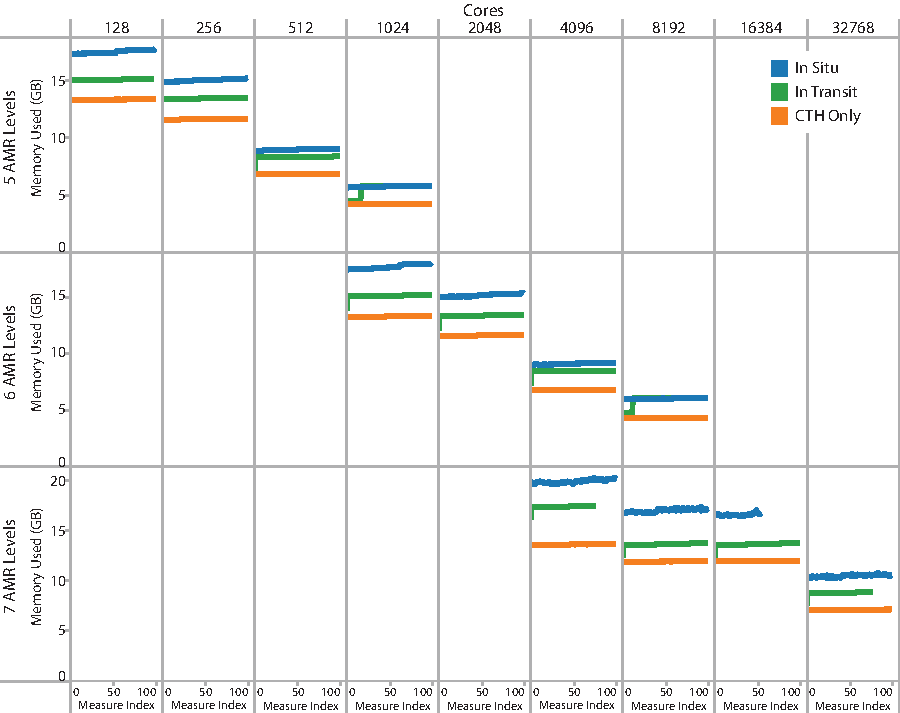
\includegraphics[width=\linewidth]{figures/MemoryUsageAll}
  \caption{Matrix of all measurements taken for memory usage comparisons.
    Each measurement is the total memory in use in a node (so for \insitu and
    \intransit memory includes both CTH simulation and overhead).  Each
    measurement is plotted as the maximum memory use in all nodes at the
    time the measurement was taken.}
  \label{fig:MemoryUsageAll}
\end{figure}

Figure~\ref{fig:MemoryInSituPerNode} gives a summary of the extra memory
used when using Catalyst for \insitu analysis during our experiments.
Likewise, Figure~\ref{fig:MemoryInTransitPerNode} gives the same summary
for the \intransit memory overhead for the nodes within the simulation
(memory usage on the separate analysis job is not given).  In all cases the
added overhead is less than 50\% than the memory used by CTH itself, and in
most cases the additional overhead is significantly smaller than that.

\begin{figure}[htb]
  \centering
  \includegraphics[width=\linewidth]{figures/MemoryUsageInSituPerNode}
  \caption{Plot of average per node memory usage of the \insitu run on Cielo.}
  \label{fig:MemoryInSituPerNode}
\end{figure}

\begin{figure}[htb]
  \centering
  \includegraphics[width=\linewidth]{figures/MemoryUsageInTransitPerNode}
  \caption{Plot of average per node memory usage of the \intransit run on Cielo.}
  \label{fig:MemoryInTransitPerNode}
\end{figure}

Figure~\ref{fig:MemoryCompare} compares the amount of memory per node added
when using \insitu versus \intransit.  As expected, the \intransit approach
requires a smaller memory overhead than \insitu within the nodes of the
simulation.  Thus, \intransit could be a better option when the simulation
requires as much memory per process as possible, but the \intransit
approach also requires separate nodes to be reserved for the analysis,
which also may cause the total amount of available simulation memory to be
reduced if nodes must be taken away from the simulation.

\begin{figure}[htb]
  \centering
  \includegraphics[width=\linewidth]{figures/MemoryUsageCompare}
  \caption{Plot of the average overhead per node of both \insitu and \intransit}
  \label{fig:MemoryCompare}
\end{figure}


